\section{Classification introduction}

\subsection{Problem contextualization}
\begin{frame}
    \frametitle{Goal of classification}

    The goal in classification is to take an input vector $x$ an 
    assign it to one of the the $K \in \N$ discrete classes 
    $\mathcal{C}_k$ where $k \in \{1, \ldots, K\}.$

    Some properties: 

    \begin{itemize}
        \item In the most common scenario, the classes are taken to be disjoint. 
        \item The input space is thereby dividen into \textit{decision regions} whose boundaries are called \textit{decision boundaries} or surfaces. 
    \end{itemize}
    If we consider linear models for classification, the decisión surface are linear functions of the input vector $x \in \R^D$, 
    and hence are defined by $(D-1)$-dimensional hyperplanes.      

\end{frame}

% Página 178
\begin{frame}
    \frametitle{Problem formulation}

    \begin{itemize}
        \item Probabilistic models: $K = 2$, two-class problems where: 
        \begin{itemize}
            \item There is a single target variable 
            $$t \in \{0,1\}$$ 
            \item Class $C_1$ is represented by $t= 1$,
            \item Class $C_2$ is represented by $t= 0$. 
            \item We can interpret the value of $t$ as the probability of class $C_1$ taking only extreme values $\{0,1\}$.
        \end{itemize}

        \item For $K > 2$ classes : \textbf{1 - of- K} coding scheme: 
        $$t \in \{0,1\}^{K} \text{where one only appears one time. }$$
    \end{itemize}
\end{frame}

\begin{frame}
    \frametitle{Distinct appraches to the classification problem}

    \begin{itemize}
        \item Constructing a \textbf{\textit{discriminant function}} that directly assigns each vector $x$ to a specific class. 
        \item Using $p(C_k | x)$ \textit{parametric function}.
        \item Using $p(C_k | x)$ with a generative approach. 
    \end{itemize}
\end{frame}

\subsection{Math formulation}
\begin{frame}
    \frametitle{Math formulation}
    We consider a generalization of lineal model, for which we 
    transform the linear function of $w$ using a nonlinear function $f$

    \begin{equation}
        y(x) = f( w^t x + w_0).
    \end{equation}

\begin{itemize}
        \item In machine learning literature $f$ is known as 
        \ti{activation function}.
        \item In statistics literature. The \ti{link function} provides the relationship between the linear predictor 
        and the mean of the distribution function \footnote{Read \cite{link_function}}, its inverse.
    \end{itemize}
\end{frame}

\section{ Discriminant Function}
\begin{frame}
    \frametitle{Discriminant functio a geometrical understanding}
    A discriminant is a function that takes an input vector $x$ and assigns it to one of $K$ classes denoted by $C_k$. 

    We shall restrict attention to \ti{linear discriminats} (decision surface are hyperplanes). 

    \textbf{Two classes }

    \begin{equation}
        y(x) = w^T x + w_0
    \end{equation}
    where 
    \begin{itemize}
        \item $w$ is called \ti{weight vector}. 
        \item $w_0$ is a \ti{bias}
    \end{itemize}
The decision boundary is defined by the relation 
\begin{equation}
    y(x) = 0
\end{equation}.  
\end{frame}

\begin{frame}
    \frametitle{$w$ determines the orientation of the decision surface}

    \begin{theorem}
        The vector $w$ is orthogonal to every vector lying within the decision surface. 
    \end{theorem}
    {\small
    \begin{proof}
        Let $v$ a vector lying within the decision surface, it can be write as the difference of two point 
        \begin{equation}
            v = v_1 - v2. 
        \end{equation}
        Those points verify that
        \begin{equation}
            y(v_i) = w ^t v_i + w_0 = 0, 
        \end{equation}
        Hence 
        \begin{equation}
            0 = y(v_1) - y(v_2) = w ^t (v_1 - v_2).
        \end{equation}
    \end{proof}
    }
\end{frame}

\begin{frame}
    \frametitle{The bias parameter $w_0$ determines the location of the deision surface}
    \begin{theorem}
        The normal distance from the origin to the decision surface is given by
        \begin{equation}
          \frac{w ^T x}{\|w\|} = - \frac{w_0}{\|w\|}.  
        \end{equation}
    \end{theorem}
    
\end{frame}

\section{Multiple classes}
\begin{frame}
    \frametitle{Multiple classes: By two class discriminant functions}

    \textit{One versus the rest} classifier has a problem: 
    leads to regions of input space that are ambiguously classified. 

    \begin{figure}[t]
        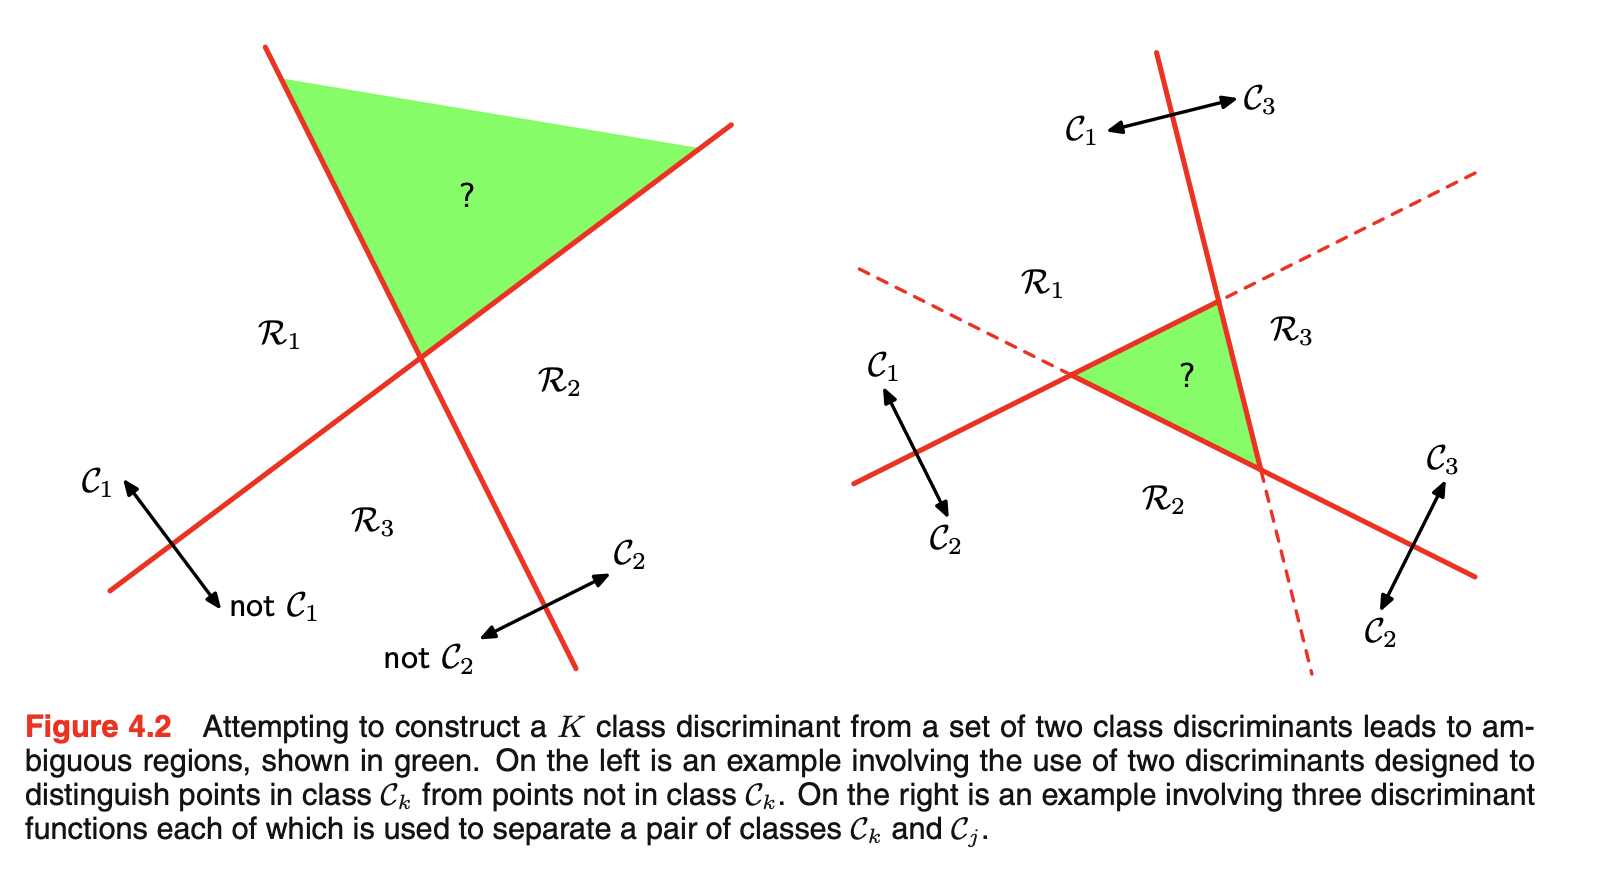
\includegraphics[height=0.7\textheight]{04_Classification/ambiguosly-one-versus-rest.png}
        \centering
    \end{figure}
\end{frame}
\begin{frame}
    \frametitle{Alternative: \ti{One versus one classifier} }
    Each  point is classified according to a majory amongst the discriminant function. 
One for ever $k (k-1) / 2$ binary discriminat functions . 

Problem: This too runs into the problem of ambiguous regions. 
\end{frame}

\begin{frame}
    \frametitle{K- Class discriminant}
Comprising $K$ linear functions of the form 

\begin{equation}
    y_k(x) = w^T_k x + w_{k0}
\end{equation}
and the assigning a point $x$ to class $C_k$
if 
\begin{equation}
    y_k(x) > y_j(x) \text{ for all  } j \neq k.
\end{equation}

The decision boundary between class $C_k$ and class $C_j$ is therefore 
given by $y_k(x) = y_j(x)$ and hence 
correspond to a $(D-1)$dimensional hyperplane 
\begin{equation}
    (w_k - w_j)^T x 
    +
    (w_{k0} - w_{j0})
    = 
    0.
\end{equation}

\end{frame}

\begin{frame}
    \frametitle{Properties}
    \begin{itemize}
        \item Regions of such a discriminant are always singly connected and convex. 
    \end{itemize}
    Let $x_a, x_b$ two points both of which lie inside decision region. 
    Any point $\hat x$ that lies on the line 
can be expressed in the form 
\begin{equation}
    \hat x = 
    \lambda x_a +
    (1- \lambda) x_b
\end{equation}
where $0 \leq \lambda \leq 1.$ 

It follows that 
\begin{equation}
    y_k( \hat{x})
    = 
    \lambda y_k(x_a)
    +
    (1- \lambda) y_k(x_b). 
\end{equation}
\end{frame}



